\documentclass{standalone}
\usepackage{tikz}
\usetikzlibrary{patterns, positioning}
\usepackage[sfdefault]{ClearSans} %% option 'sfdefault' activates Clear Sans as the default text font
\usepackage[T1]{fontenc}

\begin{document}
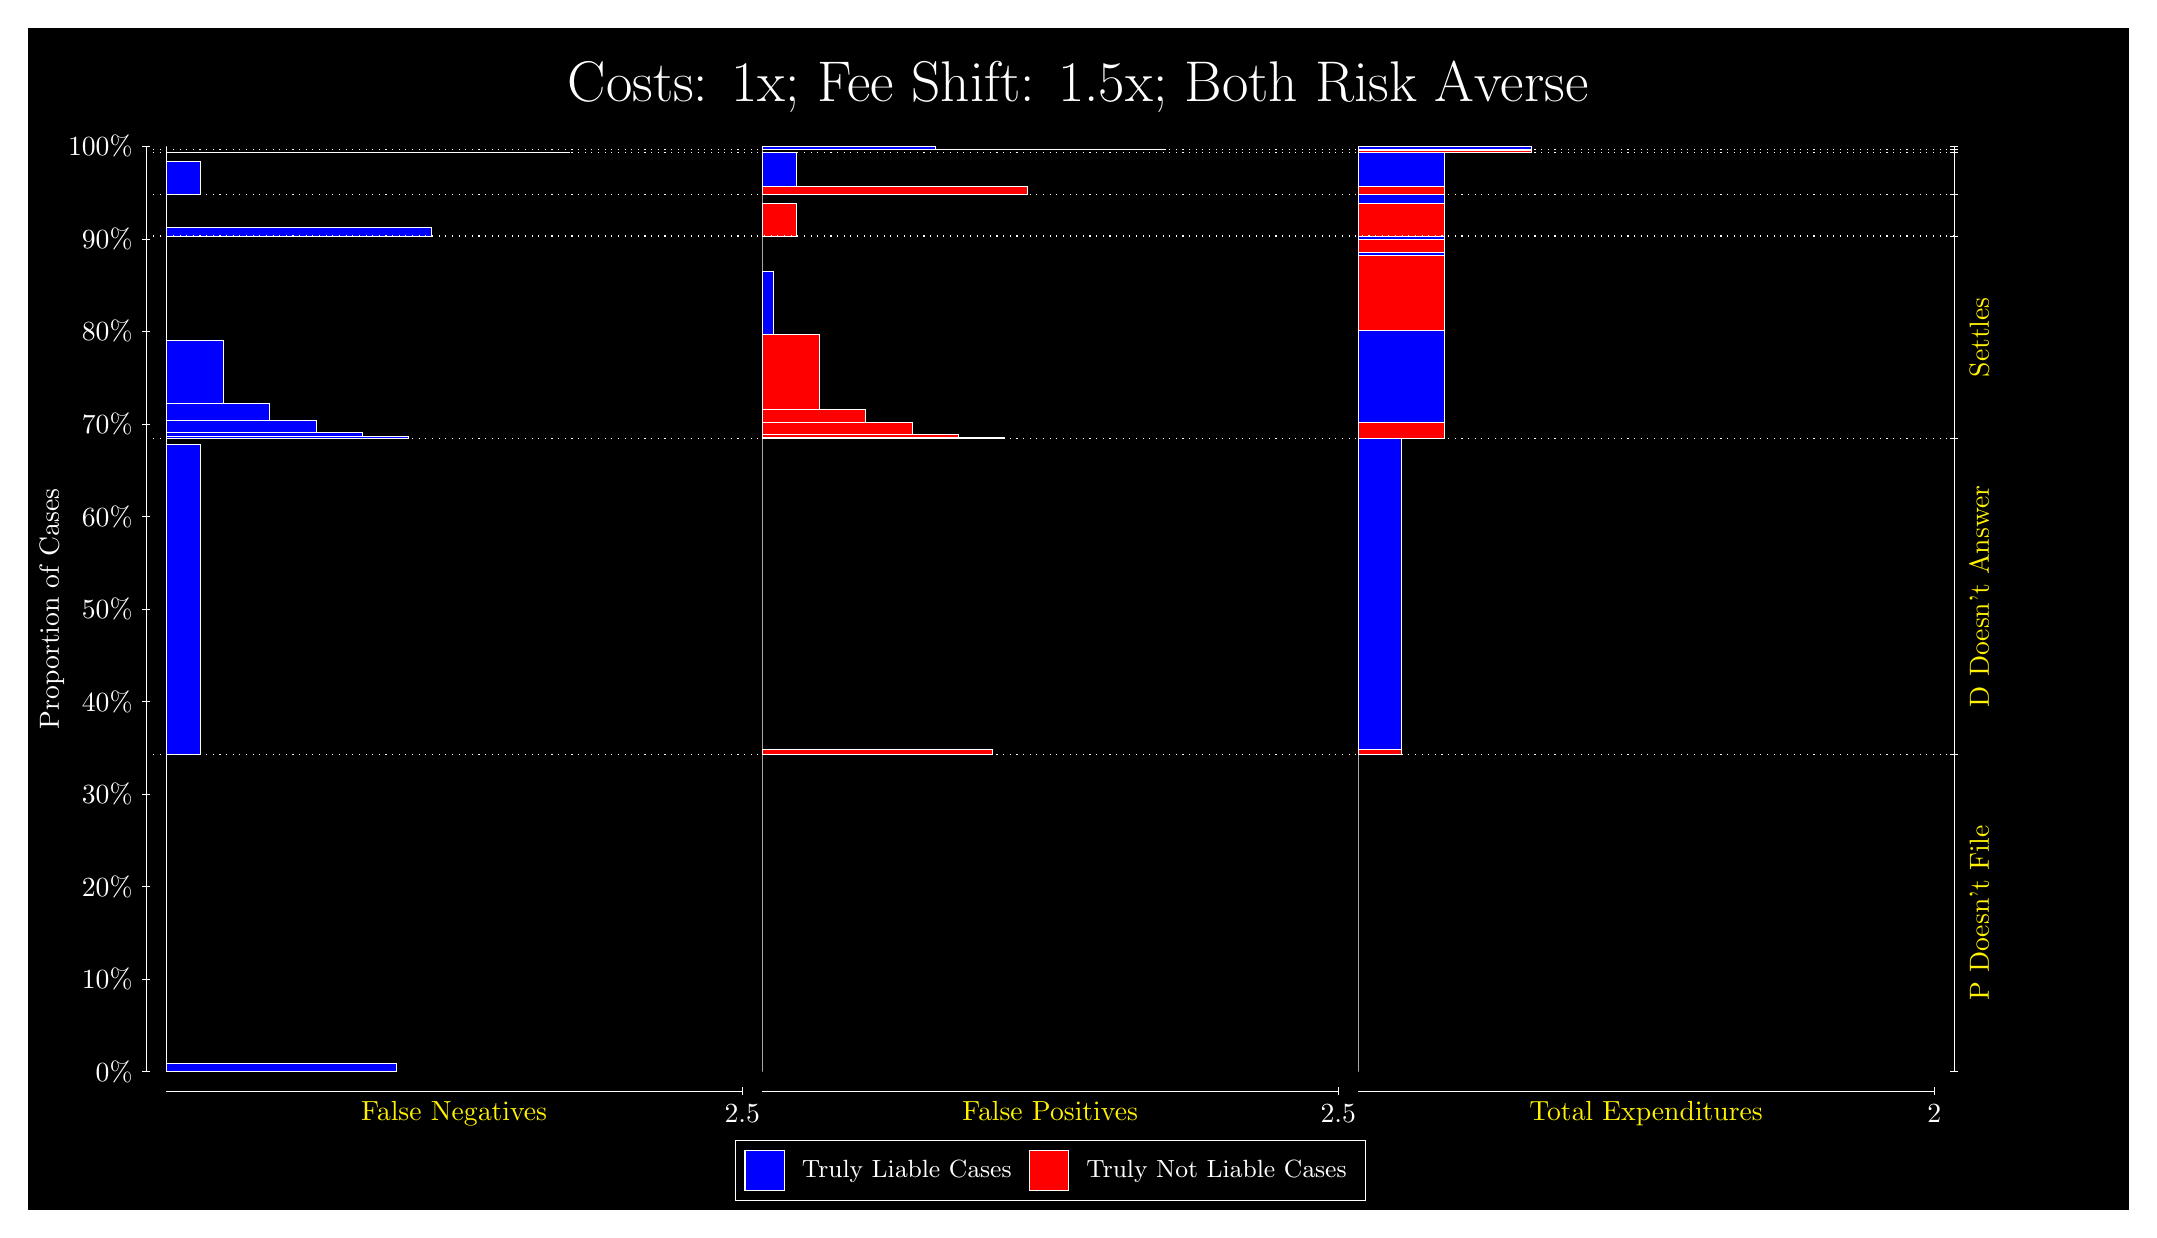
\begin{tikzpicture}
\draw[fill=black] (0,0) rectangle (26.667,15);
\draw[text=white] (0,13.5) rectangle (26.667,15) node[midway] {\huge Costs: 1x; Fee Shift: 1.5x; Both Risk Averse};
\draw[white, very thin] (1.5,1.75) -- (1.5,13.5);
\node[rotate=90, text=white, anchor=center] at (0.3, 7.625) {Proportion of Cases};
\draw[white, very thin] (1.45,1.75) -- (1.55,1.75);
\node[text=white, anchor=east] at (1.45, 1.75) {0\%};
\draw[white, very thin] (1.45,2.925) -- (1.55,2.925);
\node[text=white, anchor=east] at (1.45, 2.925) {10\%};
\draw[white, very thin] (1.45,4.1) -- (1.55,4.1);
\node[text=white, anchor=east] at (1.45, 4.1) {20\%};
\draw[white, very thin] (1.45,5.275) -- (1.55,5.275);
\node[text=white, anchor=east] at (1.45, 5.275) {30\%};
\draw[white, very thin] (1.45,6.45) -- (1.55,6.45);
\node[text=white, anchor=east] at (1.45, 6.45) {40\%};
\draw[white, very thin] (1.45,7.625) -- (1.55,7.625);
\node[text=white, anchor=east] at (1.45, 7.625) {50\%};
\draw[white, very thin] (1.45,8.8) -- (1.55,8.8);
\node[text=white, anchor=east] at (1.45, 8.8) {60\%};
\draw[white, very thin] (1.45,9.975) -- (1.55,9.975);
\node[text=white, anchor=east] at (1.45, 9.975) {70\%};
\draw[white, very thin] (1.45,11.15) -- (1.55,11.15);
\node[text=white, anchor=east] at (1.45, 11.15) {80\%};
\draw[white, very thin] (1.45,12.325) -- (1.55,12.325);
\node[text=white, anchor=east] at (1.45, 12.325) {90\%};
\draw[white, very thin] (1.45,13.5) -- (1.55,13.5);
\node[text=white, anchor=east] at (1.45, 13.5) {100\%};

\draw[white, very thin] (24.457,1.75) -- (24.457,13.5);
\draw[white, very thin] (24.407,1.75) -- (24.507,1.75);
\node[anchor=west] at (24.407, 1.75) {};
\draw[white, very thin] (24.407,5.777) -- (24.507,5.777);
\node[anchor=west] at (24.407, 5.777) {};
\draw[white, very thin] (24.407,9.7899) -- (24.507,9.7899);
\node[anchor=west] at (24.407, 9.7899) {};
\draw[white, very thin] (24.407,12.361) -- (24.507,12.361);
\node[anchor=west] at (24.407, 12.361) {};
\draw[white, very thin] (24.407,12.889) -- (24.507,12.889);
\node[anchor=west] at (24.407, 12.889) {};
\draw[white, very thin] (24.407,13.421) -- (24.507,13.421);
\node[anchor=west] at (24.407, 13.421) {};
\draw[white, very thin] (24.407,13.459) -- (24.507,13.459);
\node[anchor=west] at (24.407, 13.459) {};
\draw[white, very thin] (24.407,13.5) -- (24.507,13.5);
\node[anchor=west] at (24.407, 13.5) {};

\draw[white, very thin, fill=blue] (1.75,1.75) rectangle (4.6775,1.859);
\draw[white, very thin, fill=red] (1.75,1.859) rectangle (1.75,5.777);
\draw[white, very thin, fill=blue] (1.75,5.777) rectangle (2.1891,9.7191);
\draw[white, very thin, fill=red] (1.75,9.7191) rectangle (1.75,9.7899);
\draw[white, very thin, fill=blue] (1.75,9.7899) rectangle (4.8239,9.8222);
\draw[white, very thin, fill=blue] (1.75,9.8222) rectangle (4.2384,9.8623);
\draw[white, very thin, fill=blue] (1.75,9.8623) rectangle (3.6529,10.026);
\draw[white, very thin, fill=blue] (1.75,10.026) rectangle (3.0674,10.234);
\draw[white, very thin, fill=blue] (1.75,10.234) rectangle (2.4819,11.035);
\draw[white, very thin, fill=red] (1.75,11.035) rectangle (1.75,12.361);
\draw[white, very thin, fill=blue] (1.75,12.361) rectangle (5.1167,12.472);
\draw[white, very thin, fill=red] (1.75,12.472) rectangle (1.75,12.889);
\draw[white, very thin, fill=blue] (1.75,12.889) rectangle (2.1891,13.316);
\draw[white, very thin, fill=red] (1.75,13.316) rectangle (1.75,13.421);
\draw[white, very thin, fill=blue] (1.75,13.421) rectangle (6.8732,13.427);
\draw[white, very thin, fill=red] (1.75,13.427) rectangle (1.75,13.459);
\draw[white, very thin, fill=red] (1.75,13.459) rectangle (1.75,13.465);
\draw[white, very thin, fill=blue] (1.75,13.465) rectangle (1.75,13.5);
\draw[white, very thin, fill=red] (9.3189,1.75) rectangle (9.3189,5.668);
\draw[white, very thin, fill=blue] (9.3189,5.668) rectangle (9.3189,5.777);
\draw[white, very thin, fill=red] (9.3189,5.777) rectangle (12.246,5.8478);
\draw[white, very thin, fill=blue] (9.3189,5.8478) rectangle (9.3189,9.7899);
\draw[white, very thin, fill=red] (9.3189,9.7899) rectangle (12.393,9.8028);
\draw[white, very thin, fill=red] (9.3189,9.8028) rectangle (11.807,9.843);
\draw[white, very thin, fill=red] (9.3189,9.843) rectangle (11.222,9.993);
\draw[white, very thin, fill=red] (9.3189,9.993) rectangle (10.636,10.164);
\draw[white, very thin, fill=red] (9.3189,10.164) rectangle (10.051,11.115);
\draw[white, very thin, fill=blue] (9.3189,11.115) rectangle (9.4652,11.917);
\draw[white, very thin, fill=blue] (9.3189,11.917) rectangle (9.3189,12.361);
\draw[white, very thin, fill=red] (9.3189,12.361) rectangle (9.758,12.779);
\draw[white, very thin, fill=blue] (9.3189,12.779) rectangle (9.3189,12.889);
\draw[white, very thin, fill=red] (9.3189,12.889) rectangle (12.686,12.994);
\draw[white, very thin, fill=blue] (9.3189,12.994) rectangle (9.758,13.421);
\draw[white, very thin, fill=red] (9.3189,13.421) rectangle (9.3189,13.453);
\draw[white, very thin, fill=blue] (9.3189,13.453) rectangle (9.3189,13.459);
\draw[white, very thin, fill=red] (9.3189,13.459) rectangle (14.442,13.465);
\draw[white, very thin, fill=blue] (9.3189,13.465) rectangle (11.515,13.5);
\draw[white, very thin, fill=red] (16.888,1.75) rectangle (16.888,5.668);
\draw[white, very thin, fill=blue] (16.888,5.668) rectangle (16.888,5.777);
\draw[white, very thin, fill=red] (16.888,5.777) rectangle (17.437,5.8478);
\draw[white, very thin, fill=blue] (16.888,5.8478) rectangle (17.437,9.7899);
\draw[white, very thin, fill=red] (16.888,9.7899) rectangle (17.986,9.993);
\draw[white, very thin, fill=blue] (16.888,9.993) rectangle (17.986,11.166);
\draw[white, very thin, fill=red] (16.888,11.166) rectangle (17.986,12.118);
\draw[white, very thin, fill=blue] (16.888,12.118) rectangle (17.986,12.15);
\draw[white, very thin, fill=red] (16.888,12.15) rectangle (17.986,12.321);
\draw[white, very thin, fill=blue] (16.888,12.321) rectangle (17.986,12.361);
\draw[white, very thin, fill=red] (16.888,12.361) rectangle (17.986,12.779);
\draw[white, very thin, fill=blue] (16.888,12.779) rectangle (17.986,12.889);
\draw[white, very thin, fill=red] (16.888,12.889) rectangle (17.986,12.994);
\draw[white, very thin, fill=blue] (16.888,12.994) rectangle (17.986,13.421);
\draw[white, very thin, fill=red] (16.888,13.421) rectangle (19.083,13.453);
\draw[white, very thin, fill=blue] (16.888,13.453) rectangle (19.083,13.459);
\draw[white, very thin, fill=red] (16.888,13.459) rectangle (19.083,13.465);
\draw[white, very thin, fill=blue] (16.888,13.465) rectangle (19.083,13.5);
\draw[white, dotted] (1.5,5.777) -- (24.457,5.777);
\draw[white, dotted] (1.5,9.7899) -- (24.457,9.7899);
\draw[white, dotted] (1.5,12.361) -- (24.457,12.361);
\draw[white, dotted] (1.5,12.889) -- (24.457,12.889);
\draw[white, dotted] (1.5,13.421) -- (24.457,13.421);
\draw[white, dotted] (1.5,13.459) -- (24.457,13.459);
\draw[white, very thin] (1.75,1.5) -- (9.0689,1.5);
\node[text=yellow, anchor=north] at (5.4094, 1.5) {False Negatives};
\draw[white, very thin] (9.0689,1.45) -- (9.0689,1.55);
\node[text=white, anchor=north] at (9.0689, 1.45) {2.5};

\draw[white, very thin] (9.3189,1.5) -- (16.638,1.5);
\node[text=yellow, anchor=north] at (12.978, 1.5) {False Positives};
\draw[white, very thin] (16.638,1.45) -- (16.638,1.55);
\node[text=white, anchor=north] at (16.638, 1.45) {2.5};

\draw[white, very thin] (16.888,1.5) -- (24.207,1.5);
\node[text=yellow, anchor=north] at (20.547, 1.5) {Total Expenditures};
\draw[white, very thin] (24.207,1.45) -- (24.207,1.55);
\node[text=white, anchor=north] at (24.207, 1.45) {2};

\node[text=yellow, centered, rotate=90] at (24.777, 3.7635) {P Doesn't File};
\node[text=yellow, centered, rotate=90] at (24.777, 7.7834) {D Doesn't Answer};
\node[text=yellow, centered, rotate=90] at (24.777, 11.075) {Settles};





\draw (12.978300999999998,1.5) node[draw=none] (baseCoordinate) {};
\begin{scope}[align=center]
        \matrix[scale=0.5, draw=white, below=0.5cm of baseCoordinate, nodes={draw}, column sep=0.1cm]{
            \node[rectangle, draw, minimum width=0.5cm, minimum height=0.5cm, fill=blue] {}; &
            \node[draw=none, font=\small, text=white] (B) {Truly Liable Cases}; &
            \node[rectangle, draw, minimum width=0.5cm, minimum height=0.5cm, fill=red] {}; &
            \node[draw=none, font=\small, text=white] (B) {Truly Not Liable Cases}; \\
            };
\end{scope}

\end{tikzpicture}
\end{document}